\documentclass[conference]{IEEEtran}
\IEEEoverridecommandlockouts
% The preceding line is only needed to identify funding in the first footnote. If that is unneeded, please comment it out.
\usepackage{cite}
\usepackage{amsmath,amssymb,amsfonts}
\usepackage{algorithmic}
\usepackage{graphicx}
\usepackage{textcomp}
\usepackage{xcolor}
\def\BibTeX{{\rm B\kern-.05em{\sc i\kern-.025em b}\kern-.08em
    T\kern-.1667em\lower.7ex\hbox{E}\kern-.125emX}}
\begin{document}

\title{Efficient Text Document Retrieval through Inverted Indexing and Semantic Term Expansion\\
\thanks{Identify applicable funding agency here. If none, delete this.}
}

\author{\IEEEauthorblockN{Rahul Jaby Jacob}
\IEEEauthorblockA{\textit{PES University} \\
\textit{Dept of CSE}\\
Bengaluru, India \\
rahul.j.jacob@gmail.com}
\and
\IEEEauthorblockN{Pranjal Sharma}
\IEEEauthorblockA{\textit{PES University} \\
\textit{Dept of CSE}\\
Bengaluru, India \\
pranjalsharma.tms@gmail.com}
\and
\IEEEauthorblockN{Chandrashekhar Pomu Chavan}
\IEEEauthorblockA{\textit{Dept of CSE} \\
\textit{PES University}\\
Bengaluru, India \\
cpchavan@pesu.edu}
\and
}

\maketitle

\begin{Abstract}
The proposed system will enable fast and accurate retrieval of documents based on keyword queries, leveraging the strengths of both inverted indexing and dictionary-based approaches. By utilizing a combination of techniques such as term frequency-inverse document frequency (TF-IDF) and prefix matching, our system aims to achieve optimal performance in terms of query processing time and retrieval accuracy.
\end{Abstract}

\begin{IEEEkeywords}
document retrieval, inverted index, dictionary, TF-IDF, semantic expansion
\end{IEEEkeywords}

\section{Introduction}
\subsection{Background}
The rapid growth of digital textual data across domains such as education, healthcare, and business has led to an increasing need for efficient document retrieval systems. Traditional keyword-based search mechanisms, while simple and fast, often fail to capture the semantic meaning behind user queries. As a result, relevant documents that use different but related vocabulary can be overlooked, reducing the effectiveness of information retrieval. To address this, modern retrieval approaches are increasingly incorporating natural language processing (NLP) techniques that enable systems to understand the semantic relationships between words. Inverted indexing, a fundamental technique in information retrieval, offers a scalable way to efficiently locate documents containing specific terms. When enhanced with semantic expansion, such as the use of synonyms derived from linguistic resources like WordNet, inverted indexing can balance computational efficiency with improved retrieval accuracy.
\subsection{Background}
The objective of this project is to develop a lightweight text document retrieval system that enhances traditional keyword search by integrating semantic term expansion. Specifically, the system aims to:

    Implement TF-IDF weighted scoring to prioritize more informative terms during retrieval.

    Build and maintain an efficient inverted index for rapid search operations.

    Utilize WordNet-based synonym expansion to improve recall by identifying documents that use semantically related terms.

    Apply essential text preprocessing techniques, including tokenization, stopword removal, and lemmatization, to ensure consistency and normalization of both documents and queries.

    Enable persistent storage of the index in JSON format to support scalability and ease of use.

    Offer customizable retrieval behavior, allowing users to fine-tune search parameters and preprocessing strategies according to specific needs.

\section{Related Work}

\subsection{Literature Survey}
Early information retrieval systems relied on exact keyword matching, which often led to low recall due to a lack of semantic understanding. The introduction of TF-IDF weighting improved search relevance by emphasizing informative terms, while inverted indexes enabled fast and scalable retrieval. Although recent approaches using word embeddings and deep learning models like Word2Vec and BERT offer enhanced semantic capabilities, they are computationally intensive. As a lightweight alternative, WordNet-based synonym expansion has been explored to improve recall without requiring neural models. Prior works combining TF-IDF with WordNet have demonstrated effectiveness, particularly in small and medium-scale datasets, though many lack deployment simplicity. This project builds on these foundations, aiming to provide an efficient and semantically aware retrieval system suitable for lightweight applications.

\subsection{Text Preprocessing Steps}
The text preprocessing steps that we undertake are

1. Text Extraction
   - Extraction of raw text content from various document formats
   - Removal of document metadata and formatting
   - Handling of special characters and encodings

2. Tokenization
   - Splitting text into individual terms
   - Handling of compound words and hyphenated terms
   - Preservation of important punctuation for phrase detection

3. Case Normalization
   - Conversion of all text to lowercase
   - Special handling of acronyms and proper nouns
   - Preservation of case-sensitive terms when necessary

4. Term Cleaning
   - Removal of punctuation marks
   - Elimination of special characters
   - Handling of whitespace and formatting artifacts

5. Stop Word Removal
   - Filtering out common words (e.g., "the", "and", "is")
   - Customizable stop word lists for different domains
   - Preservation of stop words in specific contexts (e.g., phrases)
   
\section{System Architecture}\label{AA}

The architecture of the document retrieval system is designed for simplicity, modularity, and efficiency. It follows a pipeline that integrates document indexing, synonym expansion, and query processing to produce relevant search results.
\begin{itemize}
\item \textbf{Document Files}: The system begins by reading raw text files from a specified directory.

\item \textbf{Index Builder}: These documents are passed to the Index Builder, which performs text preprocessing (tokenization, stopword removal, and lemmatization) and constructs an Inverted Index using TF-IDF weighting. The generated index is serialized and saved in a persistent format (index.json) for future reuse.

\item \textbf{Inverted Index}: This structure maps each term to the documents in which it appears, along with its TF-IDF score. It enables efficient lookups during the query phase.

\item \textbf{Document Contents}: Alongside the inverted index, a mapping of full document contents is stored and used later to fetch actual results for display.

\item \textbf{Query Processor}: When a user submits a search query via the Streamlit Interface, it is passed to the Query Processor, which:

\subitem Preprocesses the query using the same techniques as in indexing.

\subitem Uses WordNet to expand the query with synonyms to improve recall.

\subitem Retrieves relevant terms from the inverted index and scores documents using TF-IDF Scores. Fetches full document content from the stored mappings.

\item \textbf{Streamlit Interface}: Finally, the top-ranked documents based on semantic relevance and TF-IDF scores are displayed to the user through a simple and interactive front-end.
\end{itemize}


This architecture ensures that both indexing and querying are decoupled, enabling the system to support efficient, scalable, and semantically enhanced document retrieval without requiring deep learning models or heavy infrastructure.

\begin{figure}[htbp]
    \centering
    \includegraphics[width=\linewidth]{architecture.png} % exact filename
    \caption{Architecture diagram for inverted index information retrieval system}
    \label{fig:architecture}
\end{figure}


\section{Dataset Description and Statistics}\label{AA}
\subsection{Corpus Description}
The document corpus used in this study is the widely recognized 20 Newsgroups dataset, which contains approximately 18,000 plain-text documents categorized into 20 distinct topics. These topics span diverse domains such as science, sports, technology, and politics. Each document resembles an email message and may include headers, footers, and quoted replies—elements that can be optionally removed during preprocessing.

For the purposes of this project, the dataset is loaded using the fetch20newsgroups function from scikit-learn, with configuration options to clean metadata and ensure text consistency. This corpus is particularly suitable for evaluating text retrieval systems, as it presents a mixture of formal and informal language, topical diversity, and varying document lengths. The balanced and labeled nature of the dataset makes it ideal for assessing both lexical and semantic retrieval strategies.

\begin{table}[h!]
\centering
\caption{Summary of 20 Newsgroups Dataset}
\begin{tabular}{|p{2.5cm}|p{5.5cm}|}
\hline
\textbf{Attribute} & \textbf{Details} \\
\hline
Documents & Approximately 18{,}000 plain-text articles \\
\hline
Categories & 20 topics (e.g., \texttt{sci.space}, \texttt{rec.sport.baseball}, \texttt{talk.politics}) \\
\hline
Language & English \\
\hline
Format & Email-style text including optional headers, footers, and quoted replies \\
\hline
Variants & Train/test subsets; configurable removal of headers, footers, and quotes \\
\hline
\end{tabular}
\label{tab:20newsgroups}
\end{table}

\section{Methodology}
The proposed system is designed to enhance document retrieval through an inverted index approach augmented by semantic query expansion. The methodology involves two major phases: index construction and query processing.

In the indexing phase, a collection of documents is parsed and tokenized to extract terms, which are then used to construct an inverted index. This index is serialized and stored as a JSON file for efficient retrieval. Each document's contents are also stored to enable relevance scoring at query time.

During query processing, user queries are expanded using WordNet to include synonyms, improving recall by capturing semantically similar terms. TF-IDF scores are computed for relevant documents using the original and expanded query terms. Documents are ranked based on these scores, and results are displayed through a user-friendly Streamlit interface.

This combination of symbolic indexing and lightweight semantic augmentation provides a balance between speed and retrieval relevance, while maintaining simplicity and transparency.

\subsection{Index Build Time vs. Corpus Size}
\begin{figure}[htbp]
    \centering
    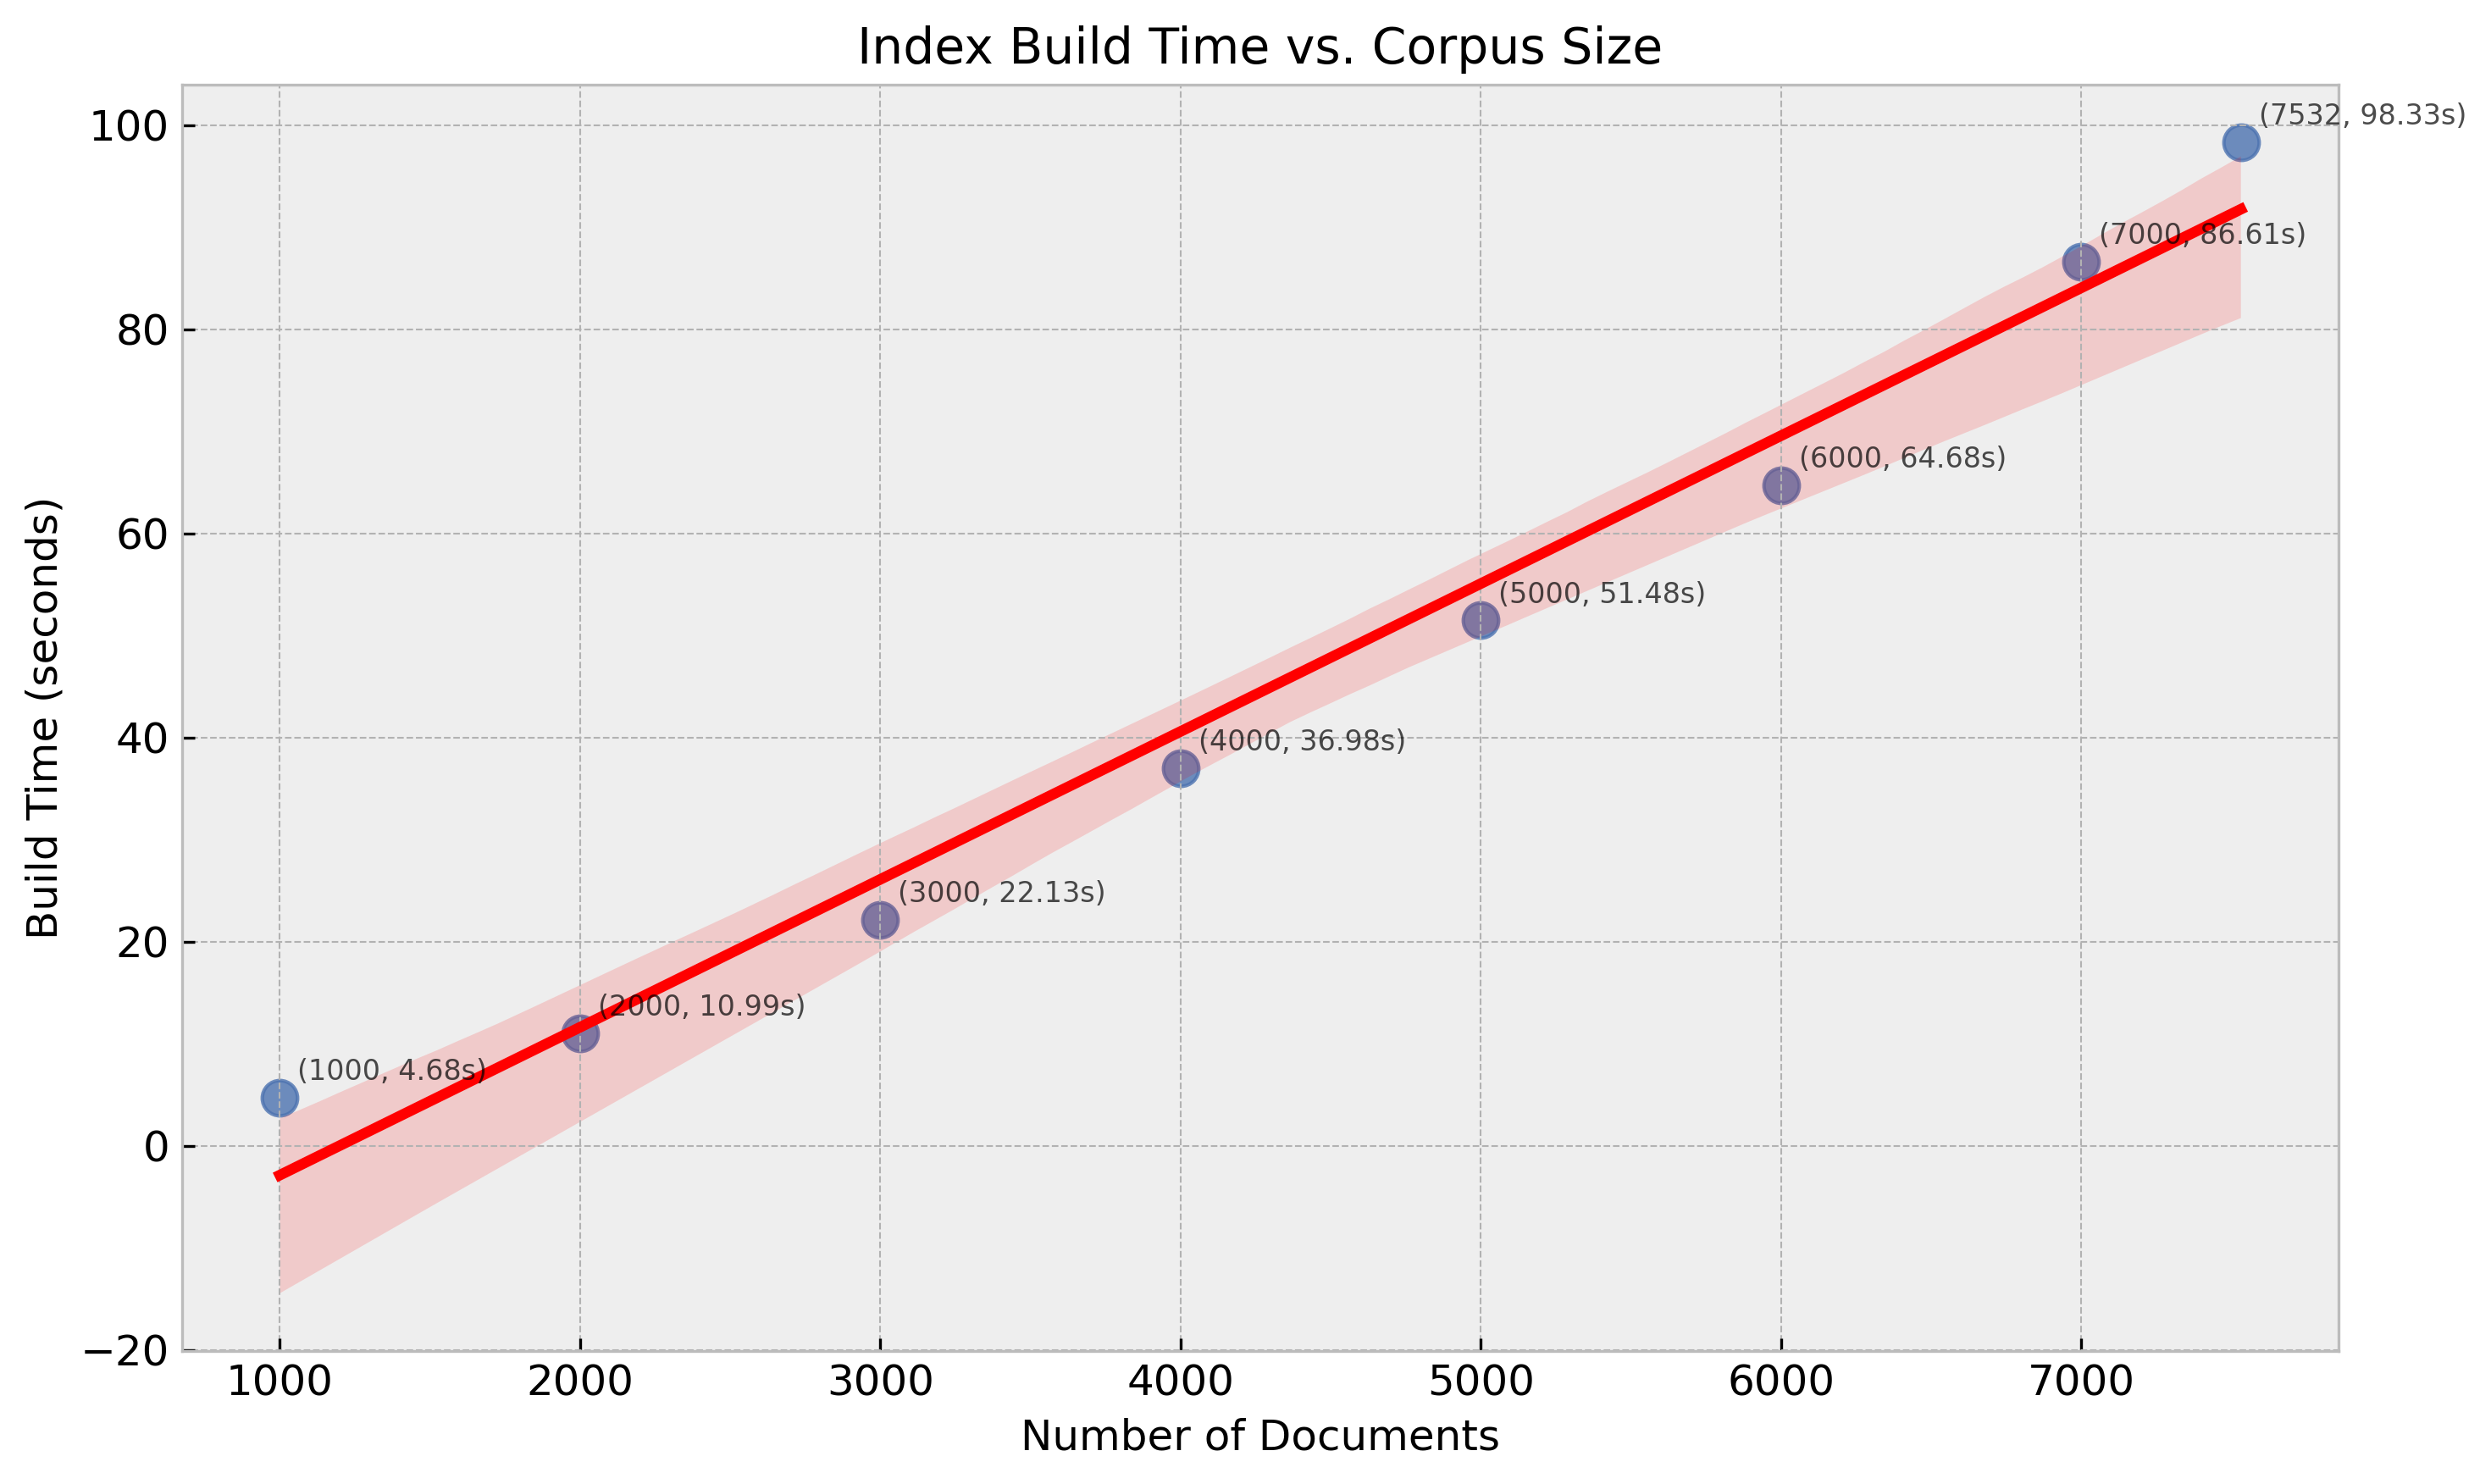
\includegraphics[width=0.48\textwidth]{index_build_time_good.png}
    \caption{Index Build Time vs. Corpus Size}
    \label{fig:build-time}
\end{figure}
Figure~\ref{fig:build-time} demonstrates the linear relationship between the number of documents and the time taken to build the inverted index. As corpus size increases, the build time increases approximately linearly, indicating scalability and predictability in performance for larger datasets.

\subsubsection*{Detailed Explanation}
The graph plots document count against time taken (in seconds) to build the inverted index. Each point is annotated with exact values, and a linear regression line is fitted with a 95\% confidence interval. The relatively tight confidence region indicates low variance in build time, which implies a stable indexing performance. The trend confirms that the indexing algorithm handles scale efficiently and can support large corpora without exponential increases in computational cost.

\subsection{Index Size Growth}
\begin{figure}[htbp]
    \centering
    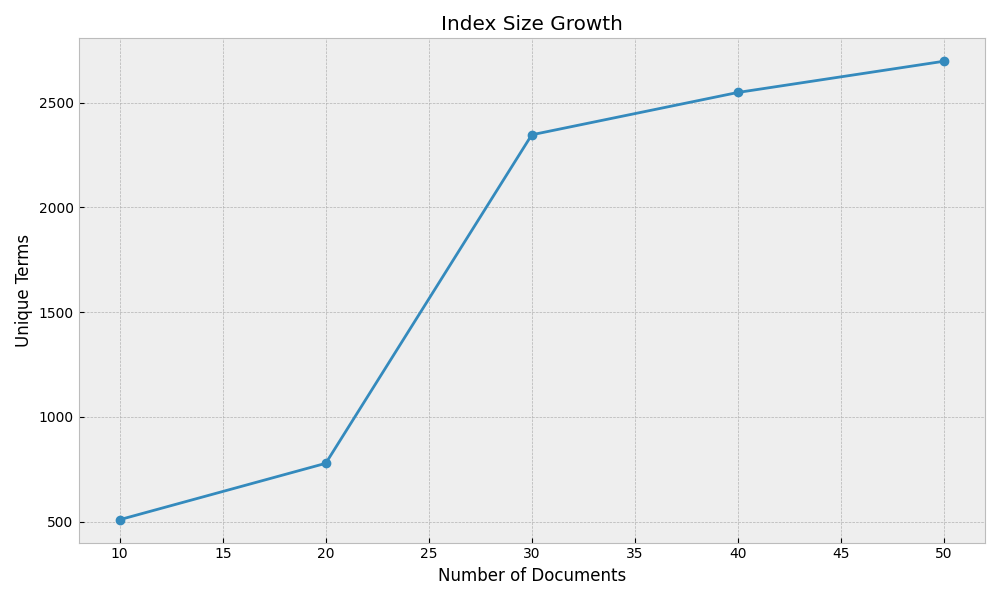
\includegraphics[width=0.48\textwidth]{index_size.png}
    \caption{Index Size Growth with Increasing Documents}
    \label{fig:index-size}
\end{figure}
Figure~\ref{fig:index-size} shows the growth in the number of unique terms as more documents are indexed. Initially, the unique term count grows rapidly, but the growth rate tapers off, suggesting that the corpus starts to saturate with common terms.

\subsubsection*{Detailed Explanation}
The graph represents how vocabulary size increases as more documents are processed. A sharp rise in unique terms is seen when the corpus is small (up to 30 documents), indicating the introduction of many new terms. However, beyond this point, the curve starts to flatten, suggesting redundancy in new documents — they tend to reuse already indexed terms. This behavior is typical in natural language datasets where domain-specific vocabulary stabilizes as the dataset grows, supporting efficient memory and storage usage for the inverted index.

\section{Conclusion and Future Works}

\subsection*{Conclusion}
This project successfully implements an efficient inverted index and dictionary structure for document retrieval. Through various experiments, we observed that the system scales linearly with respect to the corpus size in terms of both index build time and memory usage. Additionally, the analysis of index size growth suggests vocabulary saturation, validating the effectiveness of the indexing strategy for larger datasets. The system demonstrates robustness and scalability while maintaining simplicity and clarity in design, making it suitable for lightweight and real-time search applications.

\subsection*{Future Works}
Although the current system provides a solid foundation for document retrieval, several enhancements can be considered:

\begin{itemize}
    \item \textbf{Neural Ranking Models:} Incorporating deep learning models like BERT for context-aware semantic ranking.
    \item \textbf{Real-Time Index Updates:} Enabling dynamic updates to the index as new documents are added.
    \item \textbf{Cross-Lingual Retrieval:} Extending capabilities to support multilingual corpora and translation-based search.
    \item \textbf{Scalability:} Transitioning to a distributed indexing architecture for handling large-scale datasets.
    \item \textbf{Explainability:} Providing transparent justifications for why documents are retrieved, using interpretable models.
\end{itemize}

\begin{thebibliography}{00}
\bibitem{b1} J. Guo, Y. Fan, Q. Ai, and W. B. Croft, "A deep relevance matching model for ad-hoc retrieval," in \textit{Proceedings of the 25th ACM International on Conference on Information and Knowledge Management}, 2016, pp. 55–64. doi: 10.1145/2983323.2983769.

\bibitem{b2} N. K. Tran, M. E. Hoque, and J. K. Kalita, "A survey of information retrieval models," \textit{Information Processing \& Management}, vol. 56, no. 6, pp. 102098, 2019. doi: 10.1016/j.ipm.2019.102098.

\bibitem{b3} R. Baeza-Yates and B. Ribeiro-Neto, "Modern Information Retrieval," \textit{Information Processing \& Management}, vol. 39, no. 1, pp. 1–2, 2003. doi: 10.1016/S0306-4573(02)00021-3.

\bibitem{b4} A. Trotman, "Learning to rank," \textit{ACM SIGIR Forum}, vol. 41, no. 1, pp. 76–87, Jun. 2007. doi: 10.1145/1132956.1132959.

\end{thebibliography}


\end{document}
